% Provenance (never printed): see sources/outline_sources.md (Year 2: the vanished ocean;
% ophiolites; nappes; high-pressure rocks; foreland basins; reconstructing the history from
% maps, sections and geophysics). Units, ages and architecture after Schmid et al. (2004);
% Monte Cervino sheet notes (ISPRA 2016); Penrose definition as quoted by Coleman (1984);
% Zermatt-Saas ages Rubatto et al. (1998), Halama et al. (2020); Chenaillet Corno et al.
% (2023); Moho picks Michailos et al. (2023, Zenodo, CC BY 4.0); gravity Zahorec et al.
% (2021); Jura Lanza et al. (2022), Schori et al. (2015); shortening Rosenberg et al.
% (2021); Glarus thrust Herwegh et al. (2008); Molasse Krenmayr (1999), Garefalakis and
% Schlunegger (2018), Sinclair (1997); present uplift Champagnac et al. (2009). Figure data
% in figdata/bachelor-2/alps.py; exercise and problem values in the Book 4 scratch
% calculator calc/ch13.py.
\chapter{造山带剖析：阿尔卑斯山}\label{ch:b2:alpine-orogen}

马特洪峰的峰顶由片麻岩和辉长岩组成，这些岩石曾属于
阿普利亚大陆的边缘，该大陆位于已消失大洋的非洲一侧。其下的山坡
是该大洋的洋底：蛇纹岩、辉长岩和枕状玄武岩变质为榴辉岩，而
在其下方，邻近的罗莎峰之下是欧洲的边缘。沿着这一叠层向上攀登，
人便从一个大陆穿过一片大洋，抵达另一个大陆。本章把阿尔卑斯山当作这样的叠层来读：其各组成部分来自何处，它们是如何
叠置起来的，叠置吞没了多少地壳，以及地球物理在其下方看到了什么。
% ledger: ispra16:cervino, schmid04:apulia, schmid04:alpine-tethys

\begin{recall}
\textbf{来自高中分册}：大陆碰撞、缝合带、岩层的缩短
（岩层损失长度的比例）、逆断层与逆冲断层。\textbf{来自本科一年级
分册}：地质图与地质剖面；正断层、逆断层与逆冲断层、褶皱及其
指向；被动大陆边缘；洋壳、枕状熔岩与席状\omterm{def:b2:magma-emplacement:bodies}{岩墙}群；
活动大陆边缘与增生楔；均衡、艾里根与布格异常；
沉积盆地中提及的\omterm{def:b2:alpine-orogen:foreland}{前陆盆地}。\textbf{来自
\cref{ch:b2:metamorphic-facies}}：蓝片岩相与榴辉岩相。\textbf{来自
\cref{ch:b2:pt-paths}}：\omterm{def:b2:pt-paths:ptt}{P--T--t 轨迹}、\omterm{def:b2:pt-paths:exhumation}{折返速率}与\omterm{def:b2:pt-paths:uhp}{超高压
变质作用}。
\end{recall}

\begin{definition}[造山带]\label{def:b2:alpine-orogen:orogen}
称\emph{造山带}\index{造山带}为岩石圈的一个带，该带经两个板块汇聚而
缩短增厚，并包括其中经变形与变质的岩石；
山脉是其地表表现，其下增厚的地壳是其根部。
\end{definition}

\section{已消失的大洋}\label{sec:b2:alpine-orogen:tethys}

阿尔卑斯山记录了非洲板块与欧洲板块汇聚时大洋闭合的过程。
主要的是\emph{阿尔卑斯特提斯洋}，由两支构成。其南支，即
皮埃蒙特–利古里亚洋，于中侏罗世开始分离，此时中大西洋
正在张开：阿尔卑斯特提斯洋在运动学上属于大西洋的张开过程，不同于
更东边的特提斯洋。放射虫岩、深海硅质软泥固结成岩，
而 Aptychus 灰岩紧随扩张的开始出现，二者至今仍可用来指示其
残迹。北侧一支较窄，即瓦莱洋，可能张开于白垩纪
最早期。两者之间夹有一条陆块条带，即布里扬松条带，其向东
尖灭，东阿尔卑斯山中则缺失。
% ledger: schmid04:alpine-tethys

大洋北侧以欧洲的被动大陆边缘为界，该边缘是
本科一年级分册中裂谷与被动边缘一章的内容。南侧为\emph{阿普利亚}：阿尔卑斯特提斯洋以南、
新特提斯洋以北的全部陆地，包括
如今位于阿尔卑斯山以南的前陆。马特洪峰的峰顶即属于其中一部分。
% ledger: schmid04:apulia
下图标出了该\omterm{def:b2:alpine-orogen:orogen}{造山带}的位置及本章涉及的地点。

\begin{omfigure}
\centering
% ledger: data:b4-etopo-alps, schmid04:windows, schmid04:foreland, ispra16:cervino
\begin{tikzpicture}
\begin{axis}[width=0.96\linewidth, height=0.74\linewidth, xmin=5, xmax=14, ymin=43.5,
  ymax=48.5, xlabel={经度（\unit{\degree} 东）}, ylabel={纬度（\unit{\degree} 北）},
  tick label style={font=\scriptsize}, label style={font=\small}, clip=true,
  xtick={5,6,...,14}, ytick={44,45,...,48}]
\addplot[omThm!35, line width=0.3pt] table[x=lon, y=lat] {figdata/out/bachelor-2-alps-c1000.dat};
\addplot[omThm!90!black, line width=0.45pt] table[x=lon, y=lat] {figdata/out/bachelor-2-alps-c2000.dat};
\addplot[blue!60!black, line width=0.5pt] table[x=lon, y=lat] {figdata/out/bachelor-2-alps-c0.dat};
\draw[red!70!black, line width=1pt] (axis cs:8,45.3) -- (axis cs:8,48.0);
\node[font=\scriptsize\bfseries, red!70!black, anchor=north west] at (axis cs:8.02,45.32) {A};
\node[font=\scriptsize\bfseries, red!70!black, anchor=south west] at (axis cs:8.02,47.98) {B};
\fill (axis cs:6.865,45.833) circle (1.3pt) node[font=\scriptsize, fill=white, fill opacity=0.85, text opacity=1, inner sep=1pt, anchor=north east] {勃朗峰};
\fill (axis cs:7.659,45.976) circle (1.3pt) node[font=\scriptsize, fill=white, fill opacity=0.85, text opacity=1, inner sep=1pt, anchor=south east] {马特洪峰};
\node[font=\scriptsize\itshape, rotate=40] at (axis cs:6.35,46.85) {汝拉山};
\node[font=\scriptsize\itshape] at (axis cs:9.35,47.65) {磨拉石盆地};
\node[font=\scriptsize\itshape] at (axis cs:10.0,45.05) {波河平原};
\node[font=\scriptsize\itshape, align=center, fill=white, fill opacity=0.8, text opacity=1, inner sep=1pt] at (axis cs:10.3,46.95) {恩加丁 \\构造窗};
\node[font=\scriptsize\itshape, align=center, fill=white, fill opacity=0.8, text opacity=1, inner sep=1pt] at (axis cs:12.6,47.25) {陶恩 \\构造窗};
\node[font=\scriptsize\itshape] at (axis cs:8.6,43.85) {利古里亚海};
\end{axis}
\end{tikzpicture}
\par\smallskip{\small 阿尔卑斯山，取自 ETOPO1 地形模型，各节点间距 \qty{0.05}{\degree}
。等高线取 \qty{1000}{m}（浅色）与 \qty{2000}{m}（深色），并绘出海岸线。该网格的
最高节点为 \qty{3914}{m}，位于勃朗峰附近；山峰的实际海拔更高，
因为网格节点代表的是一个格元，而非山峰的顶点。沿东经 \qty{8}{\degree} 的剖线 A--B 是
本章最后一节所绘的剖面。地物名称为手工标注，位于其
大致位置。}
\end{omfigure}

已消失的大洋如何为人所知？答案在于其洋底的碎片，它们
逃脱了俯冲，被卷入\omterm{def:b2:alpine-orogen:orogen}{造山带}之中。

\begin{definition}[蛇绿岩；彭罗斯蛇绿岩序列]\label{def:b2:alpine-orogen:ophiolite}
称\emph{蛇绿岩}\index{蛇绿岩}为由镁铁质至超镁铁质岩石
构成的特征组合，即现今出露于陆地上的一段大洋岩石圈。其\emph{彭罗斯蛇绿岩
序列}\index{彭罗斯蛇绿岩序列}由地质学家会议
于 1972 年确定的完整岩石组合；自下而上依次为：
\begin{enumerate}
\item 由\omterm{def:b2:mantle-melting:peridotites}{方辉橄榄岩}、\omterm{def:b2:mantle-melting:peridotites}{二辉橄榄岩}和\omterm{def:b2:mantle-melting:peridotites}{纯橄岩}组成的超镁铁质杂岩，通常具有
在固态下获得的变形组构；
\item 辉长质杂岩，通常具有堆晶结构；
\item 镁铁质席状\omterm{def:b2:magma-emplacement:bodies}{岩墙}群；
\item 镁铁质火山杂岩，常呈枕状。
\end{enumerate}
\end{definition}
% ledger: coleman84:penrose

彭罗斯的定义是一项共识，自提出之初即受批评，
但至今仍被普遍接受。其序列即本科一年级分册中
所述的洋壳与上地幔层序：枕状熔岩覆于席状\omterm{def:b2:magma-emplacement:bodies}{岩墙}之上，席状\omterm{def:b2:magma-emplacement:bodies}{岩墙}覆于辉长岩之上，辉长岩覆于地幔之上。然而，\omterm{def:b2:alpine-orogen:ophiolite}{蛇绿岩}并非
平均意义上的洋底。大部分深海洋壳，即广阔大洋的地壳，被
俯冲所消耗。科尔曼认为，阿尔卑斯带与科迪勒拉带的\omterm{def:b2:alpine-orogen:ophiolite}{蛇绿岩}
主要形成于小洋盆的扩张中心或岛弧之间，而
特提斯带的\omterm{def:b2:alpine-orogen:ophiolite}{蛇绿岩}则形成于陆壳沿被动大陆边缘减薄、直至
一个小洋盆张开之处。
% ledger: coleman84:penrose, coleman84:settings

阿尔卑斯\omterm{def:b2:alpine-orogen:ophiolite}{蛇绿岩}符合这一图景。源自皮埃蒙特–利古里亚洋的岩片
是洋岩石圈与地幔的残块，这些地幔曾从
减薄的大陆之下被抬升、即亚大陆地幔，并出露于海底。在
西阿尔卑斯的谢纳耶，保存最好的岩片显示出露的
地幔、辉长岩及著名的枕状玄武岩序列，且无沉积盖层。
下图示出了它们。
% ledger: schmid04:units, corno23:chenaillet

\begin{omfigure}
\centering
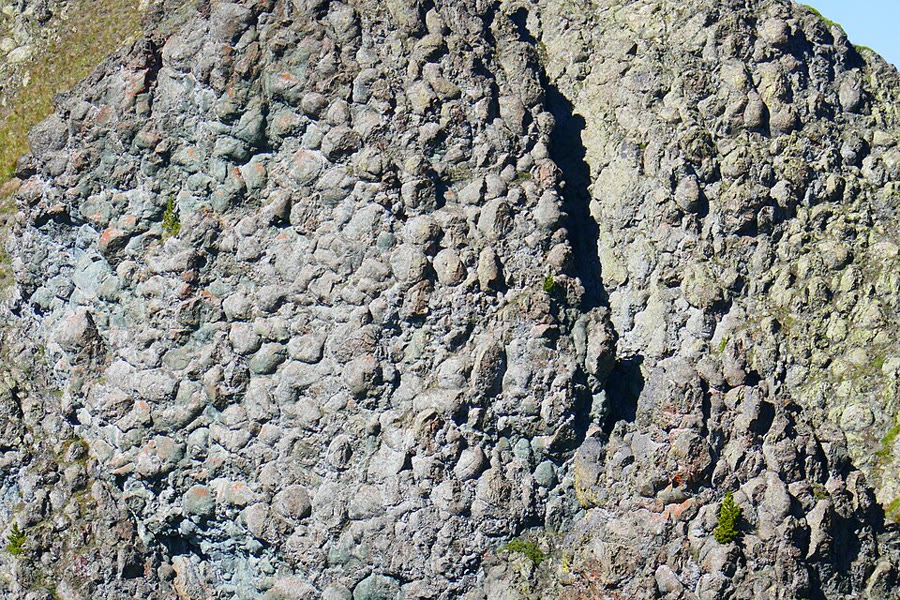
\includegraphics[width=0.66\linewidth]{images/book4/b2-13-pillow-lava.jpg}
\par\smallskip{\small 西阿尔卑斯谢纳耶\omterm{def:b2:alpine-orogen:ophiolite}{蛇绿岩}的枕状熔岩：每个圆滑的
枕体即一支玄武岩熔舌，喷发后在皮埃蒙特–利古里亚洋
底冷凝而成。照片：Lionel Duchoiselle, CC BY-SA 3.0。}
\end{omfigure}

洋底可在其辉长岩结晶处定年。两块变辉长岩的锆石，取自马特洪峰之下的
采马特–萨斯\omterm{def:b2:alpine-orogen:ophiolite}{蛇绿岩}，给出 $164.0 \pm \qty{2.7}{Ma}$ 与 $163.5
\pm \qty{1.8}{Ma}$，而覆于玄武岩之上的富锰沉积物，其年龄至多为 $161
\pm \qty{11}{Ma}$。皮埃蒙特–利古里亚洋底形成于侏罗纪，
约 \qty{164}{Ma} 前。
% ledger: rubatto98:zsf

\section{俯冲大洋，继而俯冲大陆}\label{sec:b2:alpine-orogen:subduction}

大洋通过俯冲而闭合。然而其部分洋底
却会停留在大陆之上，而非俯冲到大陆之下；也有一些大陆随洋俯冲而下。

\begin{definition}[仰冲；大陆俯冲]\label{def:b2:alpine-orogen:obduction}
\emph{仰冲}\index{仰冲}是指一片洋岩石圈板片就位于
大陆边缘之上，\omterm{def:b2:alpine-orogen:ophiolite}{蛇绿岩}骑覆于大陆之上。\emph{大陆
俯冲}\index{大陆俯冲}是指大陆岩石圈被与之相连的洋板片牵引，
下沉进入俯冲带，发生于其前方的大洋
已被消耗殆尽之后。
\end{definition}

\omterm{def:b2:alpine-orogen:obduction}{仰冲}发生于阿尔卑斯东南侧的迪纳拉山脉：侏罗纪瓦尔达尔洋的\omterm{def:b2:alpine-orogen:ophiolite}{蛇绿岩}，
本身形成于中侏罗世，于晚侏罗世被逆冲到一增生楔之上，
并逆冲到阿普利亚的大陆边缘。长期以来人们认为，谢纳耶\omterm{def:b2:alpine-orogen:ophiolite}{蛇绿岩}
同样是如此就位的，因其岩石仅显示极低级的阿尔卑斯
\omterm{def:b2:metamorphic-facies:metamorphism}{变质作用}。近期一项研究在其辉长岩与
钠长岩中发现了硬柱石与绿辉石的残留，据此将其阿尔卑斯期峰值定为 10 至 \qty{11}{kbar} 与 340 至
\qty{360}{\celsius}，相当于厚约 35 至 \qty{40}{km} 的\omterm{def:b2:alpine-orogen:nappes}{推覆体}堆的重量。作者
得出结论：谢纳耶曾被俯冲而非\omterm{def:b2:alpine-orogen:obduction}{仰冲}，这提醒人们，对\omterm{def:b2:alpine-orogen:ophiolite}{蛇绿岩}的解读
既取决于岩石，也同样取决于其变质历史。
% ledger: schmid04:obduction, corno23:chenaillet

\subsection*{大洋俯冲}

白垩纪时，皮埃蒙特–利古里亚洋南侧的阿普利亚边缘转变为一
活动大陆边缘：其海沟中充填了页岩与砂岩，今为钙质片岩，
称为 Bündnerschiefer 或 schistes lustrés。东阿尔卑斯还记录了一次更早的碰撞，
即另一大洋的海湾梅利亚塔闭合并入阿普利亚，伴随一次
高压峰值（约 \qty{100}{Ma}）：阿尔卑斯是两次造山的产物，一次
为白垩纪造山，另一次为第三纪造山。
% ledger: schmid04:two-orogenies

采马特–萨斯\omterm{def:b2:alpine-orogen:ophiolite}{蛇绿岩}曾下降至榴辉岩相（见
\cref{ch:b2:metamorphic-facies}）：其榴辉岩达 550 至 \qty{600}{\celsius} 与 2.5 至
\qty{3.0}{GPa}，峰值压力出现于 48 至 \qty{44}{Ma} 之间。其中一片，
产于奇尼亚纳湖一带，其含柯石英与微观金刚石的岩石原为玄武岩
及洋底沉积物，其温压约达 \qty{615}{\celsius} 与 \qty{2.8}{GPa}，其
锆石将该最深点定年为 $44.1 \pm \qty{0.7}{Ma}$。形成于
\qty{164}{Ma} 前的洋底，在 1.2 亿年时被俯冲至
\qty{90}{km} 或更深处，随后\omterm{def:b2:pt-paths:exhumation}{折返}。
% ledger: halama20:cignana, rubatto98:zsf

\subsection*{大陆随之俯冲}

大洋消失之后，欧洲的大陆边缘被拖拽随之而下。含柯石英的
多拉–迈拉地块石英岩（见\cref{ch:b2:pt-paths}）为大陆地壳，
来自洋的欧洲一侧，下沉深度超过 \qty{90}{km}，约
\qty{35}{Ma} 前，随后以板块速度\omterm{def:b2:pt-paths:exhumation}{折返}。对全带高压岩石的定年
给出了先后次序：阿普利亚边缘本身（塞西亚带）形成于晚
白垩世；皮埃蒙特–利古里亚洋的\omterm{def:b2:alpine-orogen:ophiolite}{蛇绿岩}约在 \qty{44}{Ma}，
欧洲大陆地壳则在晚始新世。鲁巴托及同事将其解读为三次俯冲事件，时间上由
东南向西北依次推进，朝向欧洲。
% ledger: chopin84:coesite, rh01:exhumation, rubatto98:zsf, ispra16:cervino

随后发生碰撞：作为最后一条洋带的瓦莱洋，于中至
晚始新世闭合，此后大陆地壳叠置于大陆地壳之上。
下图概括了这一序列。
% ledger: schmid04:alpine-tethys

\begin{omfigure}
\centering
\begin{tikzpicture}[x=0.95cm, y=0.78cm, font=\scriptsize]
% (a) rifting and spreading
\begin{scope}[yshift=0cm]
\node[anchor=west, font=\scriptsize\bfseries] at (-0.2,0.75) {(a) 侏罗纪：洋盆张开};
\fill[gray!25] (0,0) -- (3.2,0) -- (3.8,-0.6) -- (0,-0.6) -- cycle;
\fill[gray!25] (6.2,0) -- (10,0) -- (10,-0.6) -- (5.6,-0.6) -- cycle;
\fill[omThm!35] (3.2,0) -- (6.2,0) -- (5.6,-0.6) -- (3.8,-0.6) -- cycle;
\fill[blue!8] (0,0) rectangle (10,0.4);
\draw[thick] (4.7,0) -- (4.7,-0.6);
\node at (1.6,-0.3) {欧洲};
\node at (8,-0.3) {阿普利亚};
\node[align=center] at (4.7,0.2) {洋脊};
\end{scope}
% (b) oceanic subduction
\begin{scope}[yshift=-1.7cm]
\node[anchor=west, font=\scriptsize\bfseries] at (-0.2,0.75) {(b) 白垩纪至始新世：大洋被俯冲};
\fill[blue!8] (0,0) rectangle (7,0.4);
\fill[gray!25] (0,0) -- (3.0,0) -- (3.6,-0.6) -- (0,-0.6) -- cycle;
\fill[omThm!35] (3.0,0) -- (6.3,0) -- (6.0,-0.5) -- (5.6,-0.95) -- (3.6,-0.6) -- cycle;
\fill[gray!25] (6.3,0) -- (6.6,0.3) -- (10,0.3) -- (10,-0.6) -- (6.4,-0.6) -- cycle;
\fill[omThm!35] (5.6,-0.95) -- (6.0,-0.5) -- (7.4,-1.3) -- (7.2,-1.55) -- cycle;
\fill[orange!40] (6.0,0) -- (6.3,0) -- (6.6,0.3) -- (6.35,0.3) -- cycle;
\draw[-{Latex[length=2mm]}] (7.0,-1.0) -- (7.6,-1.38);
\node at (1.6,-0.3) {欧洲};
\node at (8.4,-0.15) {阿普利亚};
\node[anchor=west] at (7.5,-1.1) {榴辉岩};
\end{scope}
% (c) continental subduction
\begin{scope}[yshift=-3.95cm]
\node[anchor=west, font=\scriptsize\bfseries] at (-0.2,0.75) {(c) 始新世：欧洲边缘随之俯冲};
\fill[gray!25] (0,0) -- (5.6,0) -- (6.2,-0.5) -- (7.4,-1.35) -- (7.1,-1.6) -- (5.6,-0.6) -- (0,-0.6) -- cycle;
\fill[omThm!35] (6.2,0.05) -- (6.6,0.3) -- (6.95,0.3) -- (6.4,-0.2) -- cycle;
\fill[gray!25] (6.6,0.3) -- (10,0.3) -- (10,-0.6) -- (6.9,-0.6) -- (6.4,-0.2) -- (6.95,0.3) -- cycle;
\draw[dashed] (6.6,-0.85) circle (0.22);
\draw (6.82,-0.9) -- (7.6,-1.2);
\node[anchor=west] at (7.6,-1.2) {UHP 大陆地壳};
\node at (2.4,-0.3) {欧洲};
\node at (8.4,-0.15) {阿普利亚};
\end{scope}
% (d) collision
\begin{scope}[yshift=-6.65cm]
\node[anchor=west, font=\scriptsize\bfseries] at (-0.2,1.4) {(d) 渐新世至今：碰撞、推覆体与前陆盆地};
\fill[yellow!35] (0.6,0) -- (3.4,0) -- (3.4,-0.3) -- cycle;
\fill[gray!25] (0,-0.3) -- (3.4,-0.3) -- (4.2,0.5) -- (5.2,0.75) -- (6.2,0.55) -- (7.0,0.2) -- (10,0.2)
  -- (10,-0.7) -- (6.6,-0.7) -- (5.4,-1.5) -- (4.0,-1.5) -- (3.2,-0.9) -- (0,-0.9) -- cycle;
\draw (3.4,-0.3) -- (4.5,-1.0);
\draw (4.2,0.5) -- (5.6,-0.4);
\draw (5.2,0.75) -- (6.1,0.1);
\fill[omThm!35] (5.05,0.6) -- (5.55,0.68) -- (5.85,0.32) -- (5.4,0.25) -- cycle;
\fill[yellow!35] (7.0,0.2) -- (9.6,0.2) -- (7.0,-0.1) -- cycle;
\node at (1.4,-0.6) {欧洲};
\node at (8.6,-0.3) {阿普利亚};
\node[anchor=south] at (1.9,0.02) {磨拉石};
\node at (4.7,-1.25) {根};
\node[anchor=south west] at (6.25,0.6) {推覆体叠置};
\end{scope}
\end{tikzpicture}
\par\smallskip{\small 阿尔卑斯的示意演化史，非按比例绘制（洋岩石圈为红色，
大陆为灰色，增生楔为橙色，\omterm{def:b2:alpine-orogen:foreland}{前陆盆地}为黄色）。
(a)~皮埃蒙特–利古里亚洋在欧洲与阿普利亚之间张开。(b)~其洋底
俯冲至阿普利亚之下，转变为榴辉岩。(c)~欧洲大陆边缘随之被拖拽下沉，
并在超高压条件下变质。(d)~大陆地壳叠置成\omterm{def:b2:alpine-orogen:nappes}{推覆体}，覆于一
加厚的根之上，两侧发育挠曲\omterm{def:b2:alpine-orogen:foreland}{前陆盆地}。}
\end{omfigure}
% ledger: schmid04:alpine-tethys, schmid04:two-orogenies, rubatto98:zsf, schmid04:foreland

\section{推覆体、飞来峰与构造窗}\label{sec:b2:alpine-orogen:nappes}

洋与陆的碎块并非整块堆叠而成。它们被刮成薄片，
并被远距离搬运。

\begin{definition}[推覆体；推覆体叠置]\label{def:b2:alpine-orogen:nappes}
称\emph{推覆体}\index{推覆体}为一大片岩石，常厚数千米、
长数十千米，沿低角度逆冲断层或大型平卧褶皱的倒转翼，
被搬运至远离其原生位置之处。推覆体中的岩石属
\emph{外来的}\index{外来的（岩石单元）}，留在原地者属
\emph{原地的}\index{原地的（岩石单元）}。称\emph{推覆体叠置}\index{推覆体叠置}为
一堆推覆体，其中构造位置较高的
推覆体通常来自\omterm{def:b2:alpine-orogen:orogen}{造山带}更靠内侧之处。
\end{definition}

在阿尔卑斯山，叠置次序恰是已消失海洋的地理格局上下颠倒，
各单元以其来源命名（见下表）。

\begin{omfigure}
\centering\small
\begin{tabular}{>{\raggedright\arraybackslash}p{0.24\linewidth}|>{\raggedright\arraybackslash}p{0.66\linewidth}}
单元（自上而下） & 来源与岩石 \\ \hline
奥地利阿尔卑斯\omterm{def:b2:alpine-orogen:nappes}{推覆体} & 周亚得里亚线以北的阿普利亚边缘：基底与盖层
薄片，自其下地壳剥离 \\
马尼亚–塞西亚\omterm{def:b2:alpine-orogen:nappes}{推覆体}（塞西亚带，丹布朗什） & 海洋张开时自最外侧
阿普利亚边缘裂离的碎片 \\
上彭宁\omterm{def:b2:alpine-orogen:nappes}{推覆体} & 皮埃蒙特–利古里亚洋：\omterm{def:b2:alpine-orogen:ophiolite}{蛇绿岩}、\omterm{def:b2:pt-paths:exhumation}{折返}地幔、钙质
片岩 \\
中彭宁\omterm{def:b2:alpine-orogen:nappes}{推覆体} & 布里昂松带状陆块 \\
下彭宁\omterm{def:b2:alpine-orogen:nappes}{推覆体} & 瓦莱洋：\omterm{def:b2:alpine-orogen:ophiolite}{蛇绿岩}与钙质片岩 \\
亚彭宁\omterm{def:b2:alpine-orogen:nappes}{推覆体} & 欧洲基底，自其下地壳剥离 \\
赫尔维第\omterm{def:b2:alpine-orogen:nappes}{推覆体} & 近欧洲边缘富含石灰岩的盖层，与其
基底分离 \\ \hline
南阿尔卑斯 & 周亚得里亚线以南的阿普利亚：向南逆冲的\omterm{def:b2:alpine-orogen:ftb}{褶皱–冲断带}，
主要为中新世，厚 10 至 \qty{15}{km}
\end{tabular}
\par\smallskip{\small 阿尔卑斯的主要构造单元，自构造上层
向下排列，并注明各单元的来源区（据施密德等）。}
\end{omfigure}
% ledger: schmid04:units, schmid04:apulia

上盘阿普利亚位于最上部，其下依次为远侧洋、
布里昂松带、近侧洋与欧洲边缘，最底部的单元为
最靠近欧洲的单元。使\omterm{def:b2:alpine-orogen:nappes}{推覆体}在叠置后再次褶皱的大型褶皱，
有时会打乱这一次序，某些薄片如布里昂松带则
沿\omterm{def:b2:alpine-orogen:orogen}{造山带}尖灭。
% ledger: schmid04:units, schmid04:alpine-tethys

侵蚀随后切割\omterm{def:b2:alpine-orogen:nappes}{推覆体叠置}，地图上随之出现两种形态。

\begin{definition}[飞来峰；构造窗]\label{def:b2:alpine-orogen:klippe}
称\emph{飞来峰}\index{飞来峰}为\omterm{def:b2:alpine-orogen:nappes}{推覆体}的孤立残留，
即侵蚀移去其余岩席后，残留在其下岩石之上的部分；它
四周为其底部逆冲断层所包围。称\emph{构造窗}\index{构造窗}为
经侵蚀穿透\omterm{def:b2:alpine-orogen:nappes}{推覆体}所形成的洞口，其底部逆冲断层之下的岩石
由此出露，并被\omterm{def:b2:alpine-orogen:nappes}{推覆体}所环绕。
\end{definition}

\begin{omfigure}
\centering
\begin{tikzpicture}[x=0.68cm, y=0.68cm, font=\scriptsize]
\def\thrust{(0,0) -- (5,0) .. controls (6.5,0) and (7,1.1) .. (8,1.1)
  .. controls (9,1.1) and (9.5,0) .. (11,0) -- (16,0)}
\def\topo{(0,1.7) .. controls (3,1.9) and (5,1.8) .. (6,1.5) .. controls (7,1.0) .. (8,0.6)
  .. controls (9,1.0) .. (10.3,1.5) .. controls (11.3,1.3) .. (12.5,-0.4)
  .. controls (13.3,0.9) .. (14.5,0.95) .. controls (15.5,0.8) .. (16,-0.2)}
\begin{scope}
\clip \topo -- (16,-2.6) -- (0,-2.6) -- cycle;
\fill[gray!20] (0,-2.6) rectangle (16,2.2);
\fill[omThm!30] \thrust -- (16,2.2) -- (0,2.2) -- cycle;
\draw[gray!55, yshift=-0.9*0.68cm] \thrust;
\draw[gray!55, yshift=-1.8*0.68cm] \thrust;
\draw[line width=1.2pt] \thrust;
\end{scope}
\draw \topo;
\node at (2.5,1.0) {推覆体};
\node[anchor=north west] at (0.2,-0.05) {底部逆冲断层};
\node at (3.6,-1.35) {原地岩系};
\draw[-{Latex[length=1.6mm]}] (8,2.0) node[anchor=south] {构造窗} -- (8,0.75);
\draw[-{Latex[length=1.6mm]}] (14.5,2.0) node[anchor=south] {飞来峰} -- (14.5,1.05);
\end{tikzpicture}
\par\smallskip{\small 侵蚀后，\omterm{def:b2:alpine-orogen:nappes}{推覆体}（彩色）覆于其原地岩系（灰色）之上的
示意剖面：其底部逆冲断层（粗线）向上拱起处，侵蚀已切穿\omterm{def:b2:alpine-orogen:nappes}{推覆体}，
并露出其下岩石，形成\omterm{def:b2:alpine-orogen:klippe}{构造窗}；前方，\omterm{def:b2:alpine-orogen:nappes}{推覆体}的一块残留
孤立地立于原地岩系之上，即\omterm{def:b2:alpine-orogen:klippe}{飞来峰}。}
\end{omfigure}

阿尔卑斯山中两者都很多。马特洪峰是一座\omterm{def:b2:alpine-orogen:klippe}{飞来峰}：其峰顶属于丹布朗什
逆冲系，为立于整个楔体之上的阿普利亚岩石孤立残块，其
二叠纪的片麻岩与辉长岩，覆于策马特–萨斯\omterm{def:b2:alpine-orogen:nappes}{推覆体}的\omterm{def:b2:alpine-orogen:ophiolite}{蛇绿岩}之上，
及其下的孔宾带，二者依次覆于欧洲一侧的蒙特罗莎
与大圣伯纳\omterm{def:b2:alpine-orogen:nappes}{推覆体}之上（见下图）。阿尔卑斯西部北部前缘，
来自\omterm{def:b2:alpine-orogen:orogen}{造山带}深处的盖层\omterm{def:b2:alpine-orogen:nappes}{推覆体}构成了罗曼前阿尔卑斯山及
瑞士中部的\omterm{def:b2:alpine-orogen:klippe}{飞来峰}。在阿尔卑斯东部，两个\omterm{def:b2:alpine-orogen:klippe}{构造窗}穿透
奥地利阿尔卑斯盖层：恩加丁\omterm{def:b2:alpine-orogen:klippe}{构造窗}中，瓦莱洋片岩与蓝片岩
出露于布里昂松带的最后残片之下；较大的陶恩\omterm{def:b2:alpine-orogen:klippe}{构造窗}中，
欧洲边缘与阿尔卑斯特提斯洋的薄片自奥地利阿尔卑斯\omterm{def:b2:alpine-orogen:nappes}{推覆体}
之下露出。
% ledger: ispra16:cervino, schmid04:windows

\begin{omfigure}
\centering
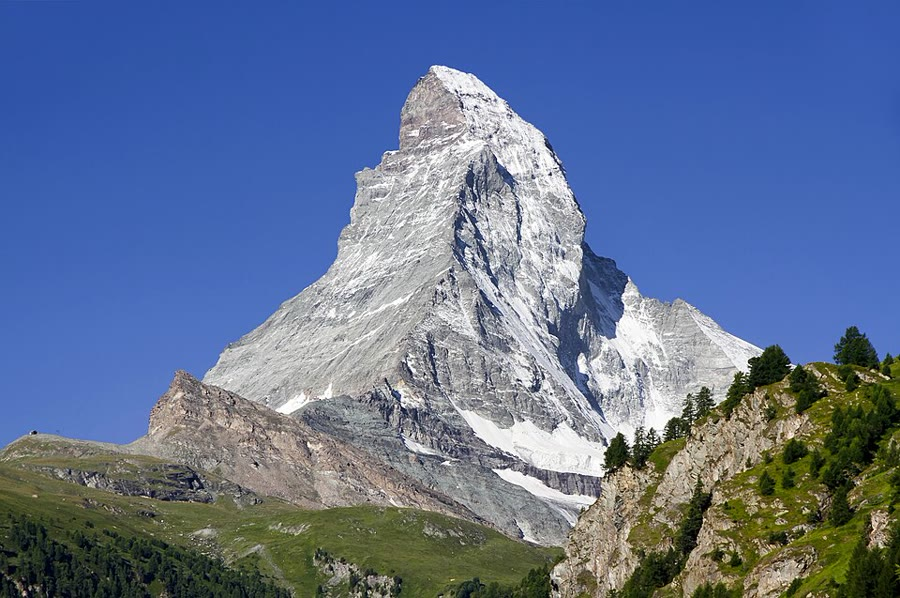
\includegraphics[width=0.7\linewidth]{images/book4/b2-13-matterhorn.jpg}
\par\smallskip{\small 从策马特望去的马特洪峰东北面（\qty{4478}{m}）：
其上部金字塔形山体为阿普利亚的片麻岩与辉长岩，属丹布朗什逆冲系，是
覆于阿尔卑斯特提斯洋\omterm{def:b2:alpine-orogen:ophiolite}{蛇绿岩}之上的\omterm{def:b2:alpine-orogen:klippe}{飞来峰}。照片：Ximonic (Simo Räsänen), CC BY-SA
4.0。}
\end{omfigure}
% ledger: ispra16:cervino

\subsection*{滑脱面与薄皮、厚皮构造}

\omterm{def:b2:alpine-orogen:nappes}{推覆体}与逆冲岩片沿软弱面运动。

\begin{definition}[滑脱面]\label{def:b2:alpine-orogen:decollement}
\emph{滑脱面}\index{滑脱面}是一个低角度面，一套岩层沿此面与下伏岩层分离，
并沿其滑动，两侧各自独立变形；
它通常沿蒸发岩或页岩等软弱层发育。
\end{definition}

\begin{definition}[薄皮构造与厚皮构造]\label{def:b2:alpine-orogen:skin}
\emph{薄皮构造}\index{薄皮构造}是指一种沉积盖层的变形，
该盖层沿底部\omterm{def:b2:alpine-orogen:decollement}{滑脱面}与其基底分离，盖层发生褶皱与逆冲，
而其下伏基底不发生变形。\emph{厚皮构造}\index{厚皮构造}
是指基底也参与其中的变形，
盖层与基底沿切入基底的断层共同缩短。
\end{definition}
% ledger: lanza22:jura

\begin{definition}[褶皱–冲断带]\label{def:b2:alpine-orogen:ftb}
\emph{褶皱–冲断带}\index{褶皱–冲断带}是由褶皱和逆冲断层组成的带，
它使\omterm{def:b2:alpine-orogen:orogen}{造山带}外缘缩短，并向前陆方向扩展；逆冲断层
自\omterm{def:b2:alpine-orogen:decollement}{滑脱面}向上穿过各层抬升，褶皱则在其上方发育。
\end{definition}

阿尔卑斯山两种构造兼备。赫尔维第\omterm{def:b2:alpine-orogen:nappes}{推覆体}是薄皮\omterm{def:b2:alpine-orogen:ftb}{褶皱–冲断带}，
由靠近欧洲大陆边缘的中生代石灰岩与其基底分离而成。其底界为
格拉鲁斯逆冲断层，二叠纪红层在此覆于新生代\omterm{def:b2:alpine-orogen:foreland}{复理石}之上。中新世时则不同：
外部地块的基底岩块，即经缩短加厚的欧洲基底（阿尔、
勃朗峰、贝尔多纳、佩尔武和阿根特拉地块），连同其盖层被逆冲推起，
属厚皮逆冲。
% ledger: schmid04:units, schmid04:skins, herwegh08:glarus, rosenberg21:massifs

汝拉山脉是瑞士平原西北方的一道弧形山脊，是\omterm{def:b2:alpine-orogen:skin}{薄皮构造}的
经典例子。晚中新世与上新世时，其中生代盖层折叠，并沿
中、上三叠统软弱蒸发岩中的\omterm{def:b2:alpine-orogen:decollement}{滑脱面}逆冲推覆，而其下伏基底
未参与变形：该基底自外部地块向下延伸至\omterm{def:b2:alpine-orogen:foreland}{磨拉石}盆地之下，
依经典解释，推动力来自远处的外部地块。此后，地震学
又补充了\omterm{def:b2:alpine-orogen:skin}{厚皮构造}的一章。2000 年圣于尔桑地震的震源
不足一千米深，为逆冲型震源机制，表明盖层浅部正在逆冲；
另有研究发现，自晚上新世以来基底断层已重新活动。汝拉山脉是否仍与其基底分离，
尚有争议。
% ledger: lanza22:jura, schmid04:skins

\begin{inthefield}[读懂逆冲接触]
格拉鲁斯逆冲断层横穿瑞士东部的弗利姆斯与瓦伦湖之间，是
阿尔卑斯山最突出的大型低角度逆冲断层之一。沿其分布的二叠纪红层，即
Verrucano 层，覆于新生代\omterm{def:b2:alpine-orogen:foreland}{复理石}之上：较老的岩层压在较新的岩层之上。两者之间，一条
薄而强烈剪切的石灰岩带构成接触面，即洛赫赛滕石灰岩，位移量至少 30 至 \qty{40}{km}，集中于此。
十九世纪时，海姆将此构造解读为两个相对的巨大
倒转褶皱；埃舍尔·冯德·林特则认为只有一条逆冲断层，后一种逆冲解释占了上风。地质学家遇到此类接触时，需核查
以下三点：老岩层是否覆于新岩层之上（这是普通层理无法做到的）；
接触两侧的岩层是否在接触处被切断；
接触面本身是否为剪切并重结晶的岩石带，而非层面。
\end{inthefield}
% ledger: herwegh08:glarus

\section{前陆盆地：复理石与磨拉石}\label{sec:b2:alpine-orogen:foreland}

\omterm{def:b2:alpine-orogen:orogen}{造山带}给其所依附的板块施加荷载，板块在其前方向下弯曲。

\begin{definition}[前陆盆地；复理石；磨拉石]\label{def:b2:alpine-orogen:foreland}
\emph{前陆盆地}\index{前陆盆地}是一个长条形沉积盆地，形成于
\omterm{def:b2:alpine-orogen:orogen}{造山带}与其前方稳定大陆之间，板块在逆冲楔的荷载下向下弯曲；
该盆地在靠近逆冲前缘处最深，并且自身
逐渐被逆冲覆盖。\emph{复理石}\index{复理石}是此类盆地的深水充填物，
主要为砂岩与页岩组成的浊积岩，沉积于盆地欠充填之时。
\emph{磨拉石}\index{磨拉石}是其后期的浅海与陆相充填物，主要为
来自被侵蚀\omterm{def:b2:alpine-orogen:orogen}{造山带}的砾岩与砂岩，沉积于物源
已充满盆地之后。
\end{definition}
% ledger: sinclair97:trinity, schmid04:foreland, krenmayr99:molasse

弯曲即岩石圈的弹性挠曲，将在本科三年级的一章中讨论；
这里只关心其对盆地的影响。辛克莱将早期阿尔卑斯\omterm{def:b2:alpine-orogen:foreland}{前陆盆地}（古新世至渐新世）描述为
“欠充填三联体”：大陆一侧为石灰岩，中部为半远洋泥，
靠近逆冲前缘处为深水浊积岩。随着逆冲推进，盆地也随之
移动：在瑞士境内，其大陆岸线以每年 8.5
至 \qty{12.9}{mm} 的速度向西北推移，盆地形态近乎不变，并在
欧洲板块上迁移了至少 \qty{210}{km}。
% ledger: sinclair97:trinity

北阿尔卑斯\omterm{def:b2:alpine-orogen:foreland}{磨拉石}盆地自滨海阿尔卑斯山延伸至维也纳，于晚始新世开始
沉降。下渐新统\omterm{def:b2:alpine-orogen:foreland}{复理石}（今见于赫尔维第\omterm{def:b2:alpine-orogen:nappes}{推覆体}之上）记录了最后一个深水阶段；
自晚渐新世至晚中新世，河流
将来自年轻山脉的陆相砾石与砂铺散开来。该名称历史悠久：索絮尔于
1779 年提出\emph{\omterm{def:b2:alpine-orogen:foreland}{磨拉石}}一词。充填层向\omterm{def:b2:alpine-orogen:orogen}{造山带}方向增厚：
在逆冲前缘处厚度超过 \qty{4000}{m}（奥地利段），盆地其他处则
为一套晚渐新世河流砾岩，厚约 \qty{4}{km}。盆地南部已被推覆：奥地利段
的露头带宽约 \qty{60}{km}，不足盆地原宽度的四分之一。被推覆的\omterm{def:b2:alpine-orogen:foreland}{磨拉石}
本身卷入逆冲之中，成为亚阿尔卑斯\omterm{def:b2:alpine-orogen:foreland}{磨拉石}，即一系列
向南倾斜的砾岩岩片，沿\omterm{def:b2:alpine-orogen:orogen}{造山带}
北缘分布。
% ledger: schmid04:foreland, krenmayr99:molasse, gs18:conglomerates

阿尔卑斯山以南，波河平原位于南阿尔卑斯山的弱变形亚得里亚前陆之上。
其最年轻的上新世与更新世沉积物部分不整合地覆盖阿尔卑斯构造，
部分则受南阿尔卑斯山的最后几次逆冲变形，
也受亚平宁山脉最后逆冲的影响。
% ledger: schmid04:foreland

\begin{omfigure}
\centering
\begin{tikzpicture}[x=0.5cm, y=0.6cm, font=\scriptsize]
\begin{scope}
\node[anchor=west, font=\scriptsize\bfseries] at (0,2.4) {(a) 欠充填：复理石};
\fill[blue!8] (0,0) -- (12,0) -- (12,1.4) -- (9.0,1.4) -- (4,0.05) -- (0,0.05) -- cycle;
\fill[gray!25] (0,0) -- (12,-1.1) -- (12,-1.9) -- (0,-0.8) -- cycle;
\fill[omThm!30] (9.0,1.4) -- (12,2.2) -- (12,-1.1) -- (9.5,-0.87) -- cycle;
\fill[green!25!gray!40] (5.5,-0.5) -- (9.5,-0.87) -- (9.3,-0.35) -- (7.0,-0.2) -- cycle;
\node at (10.9,0.6) {逆冲楔};
\node at (2,-0.45) {克拉通};
\node[anchor=north] at (7.3,-0.9) {浊积岩};
\draw[->] (7.3,-0.95) -- (7.6,-0.55);
\end{scope}
\begin{scope}[xshift=6.4cm]
\node[anchor=west, font=\scriptsize\bfseries] at (0,2.4) {(b) 过充填：磨拉石};
\fill[gray!25] (0,0) -- (12,-1.1) -- (12,-1.9) -- (0,-0.8) -- cycle;
\fill[omThm!30] (8.5,1.6) -- (12,2.4) -- (12,-1.1) -- (9.0,-0.82) -- cycle;
\fill[yellow!40] (1.5,-0.13) -- (9.0,-0.82) -- (8.5,1.0) -- (5,0.35) -- cycle;
\fill[blue!8] (0,0) -- (1.5,-0.13) -- (5,0.35) -- (4,0.4) -- (0,0.4) -- cycle;
\node at (10.6,0.6) {逆冲楔};
\node at (2,-0.45) {克拉通};
\node at (6.2,-0.05) {砾石、沙};
\end{scope}
\end{tikzpicture}
\par\smallskip{\small \omterm{def:b2:alpine-orogen:foreland}{前陆盆地}的两个阶段（示意）。(a)~早期，弯曲的板块沉降
快于沉积物的供给：深水环境紧邻逆冲楔，其中
堆积浊积岩（\omterm{def:b2:alpine-orogen:foreland}{复理石}）。(b)~晚期，被侵蚀的\omterm{def:b2:alpine-orogen:orogen}{造山带}供给
的物质超过盆地所能容纳的量：河流以砾石与砂（\omterm{def:b2:alpine-orogen:foreland}{磨拉石}）充填盆地，
逆冲楔则逆冲覆盖其自身的碎屑。}
\end{omfigure}
% ledger: sinclair97:trinity, schmid04:foreland

\section{解读历史：剖面与地球物理}\label{sec:b2:alpine-orogen:sections}

地图显示各单元的位置；剖面则显示它们在地下如何排列，
并且它可以被检验。

\begin{definition}[平衡剖面]\label{def:b2:alpine-orogen:balanced}
称\emph{平衡剖面}\index{平衡剖面}为变形岩石的剖面，
沿运移方向绘制，并可在不增减岩石的前提下
复原为地质上合理的未变形状态：剖面中标志层的长度
与岩石单元的面积，在变形与复原两种状态之间
保持守恒。
\end{definition}

复原以\emph{钉线}为锚定：钉线是横穿剖面两端各岩层的线，
选在岩石未发生相互滑移的位置。

\begin{proposition}[长度与面积平衡]\label{prop:b2:alpine-orogen:balance}
在变形状态下，两条钉线相距 $l$，设某标志层
沿层测得的长度为 $l_0$，设原始厚度为 $t$ 的某一层的
截面积为 $A$。若在剖面平面内长度与面积守恒，则
\begin{enumerate}
\item 变形前该层长为 $l_0$，缩短率
为 $e = 1 - l/l_0$，缩短距离为 $S = l_0 - l$；
\item 该层复原后的长度为 $l_0 = A/t$；
\item 若某标志层位于平直\omterm{def:b2:alpine-orogen:decollement}{滑脱面}之上深度 $d$ 处，则被抬升至
标志层原始水平以上的岩石面积，即\emph{超余面积} $A_e$，等于 $S\,d$；
因此 $d = A_e/S$。
\end{enumerate}
\end{proposition}

\begin{omfigure}
\centering
% book's own geometry (figdata/bachelor-2/alps.py)
\begin{tikzpicture}
\begin{axis}[width=0.86\linewidth, height=4.0cm, axis equal image, xmin=-1.5, xmax=31.5,
  ymin=-7.5, ymax=4.8, axis lines=none, clip=false]
\addplot[omThm, line width=1.2pt] table[x=x_km, y=y_km] {figdata/out/bachelor-2-alps-chevron.dat};
\addplot[gray, line width=1.2pt] table[x=x_km, y=y_km] {figdata/out/bachelor-2-alps-chevron0.dat};
\draw[dashed] (axis cs:0,-7) -- (axis cs:0,4.3);
\draw[dashed] (axis cs:22.98,-1.2) -- (axis cs:22.98,4.3);
\draw[dashed] (axis cs:30,-7) -- (axis cs:30,-4.8);
\draw[<->] (axis cs:0,-1.4) -- node[below, font=\scriptsize] {$l = \qty{23.0}{km}$} (axis cs:22.98,-1.4);
\node[font=\scriptsize, anchor=south] at (axis cs:15,-5.9) {复原：$l_0 = \qty{30.0}{km}$};
\node[font=\scriptsize, anchor=west] at (axis cs:23.3,2.2) {翼部倾角 \qty{40}{\degree}};
\node[font=\scriptsize, anchor=south] at (axis cs:0,4.3) {钉线};
\node[font=\scriptsize, anchor=south] at (axis cs:22.98,4.3) {钉线};
\end{axis}
\end{tikzpicture}
\par\smallskip{\small 标志层长度平衡：该层褶皱成人字形，两翼
倾角为 \qty{40}{\degree}（上图），以及同一层在两条钉线间复原后的样子（下图，
按真实比例绘制）。每个翼部保持其长度；褶皱后的岩层跨度
为 $l = 30.0\cos\qty{40}{\degree} = \qty{23.0}{km}$，缩短率为 $1 - \cos\qty{40}{\degree} =
\qty{23.4}{\percent}$。}
\end{omfigure}

\begin{proof}
（1）沿长度既不伸长也不缩短的层保持其长度；缩短率
即损失长度的比例，如同中学所学。（2）变形前，该层为一条
长 $l_0$、厚 $t$、面积为 $l_0 t$ 的带状体，面积守恒。（3）变形前，
标志层与\omterm{def:b2:alpine-orogen:decollement}{滑脱面}之间的岩石充填一条长 $l_0$、厚 $d$ 的带状区域。变形后，
两钉线之间，同一岩石充填一条长 $l$ 的带状区域，从\omterm{def:b2:alpine-orogen:decollement}{滑脱面}直到标志层原始水平，
面积为 $l\,d$，加上被推升至该水平之上的超余面积。
由守恒得 $l_0 d = l\,d + A_e$，于是 $A_e = (l_0 -
l)\,d = S\,d$。由此，据测得的超余面积与缩短量，
即可求出隐伏\omterm{def:b2:alpine-orogen:decollement}{滑脱面}的深度。
\end{proof}


\begin{method}[剖面的复原]\label{met:b2:alpine-orogen:restore}
\begin{enumerate}
\item 选取平行于运移方向的剖面，以及两条层间无滑动的
位置作为钉线。
\item 沿长度在两钉线之间量取各标志层，计入
每一段因逆冲而重复出现的部分。
\item 按测得的长度将各层摊平，保持地层顺序，
并在复原剖面上重绘断层，其切割点须对齐，
不留空隙，也不重叠。
\item 比较：同一逆冲岩片中的层须复原为相同长度；各层面积
除以其厚度所得的长度也须相同。若某剖面
不满足上述要求，则所绘剖面不可接受。
\end{enumerate}
\end{method}

平衡方法是对剖面的一种检验，而非证明，其假设至关重要。在汝拉山
沙瑟拉勒附近，对侏罗系顶部做长度平衡，得到 \qty{5.1}{km} 的
位移，而面积平衡与正演模拟给出 \qty{11.3}{km}：多出的
\qty{6.2}{km} 由侏罗系页岩中的第二条上部\omterm{def:b2:alpine-orogen:decollement}{滑脱面}带走，并
传递至更北侧的褶皱。一个标志层漏计了一半的位移。同一研究
权衡了汝拉山常见的另外两种解释，并认为二者均不必要：基底隆起
推动褶皱上升，以及三叠系蒸发岩流入背斜核部使其增厚，这一
过程会破坏面积平衡，因为蒸发岩层不再保持
其厚度。
% ledger: schori15:chasseral, schori15:evaporite-flow

\subsection*{缩短量有多大？}

将平衡方法应用于整条剖面线时，可得到\omterm{def:b2:alpine-orogen:orogen}{造山带}的总体缩短量，而答案
随假设而异。沿中阿尔卑斯的 NFP-20 剖面线，碰撞缩短量的估计
在早期研究中约为 \qty{125}{km}，在 2015 年的汇编中为 \qty{160}{km}，
在 2021 年的综述中为 \qty{144}{km}；加上环亚得里亚线上的右行滑动，
该滑动使阿普利亚沿\omterm{def:b2:alpine-orogen:orogen}{造山带}侧向移动，使总体汇聚量提高至 206 与
\qty{250}{km} 之间，取决于所设定的滑动量。在西阿尔卑斯，估计值
范围为 124 至 \qty{243}{km}。这些估计值每一个都是复原片段之和，每个片段
各有其自身的钉线，以及对被侵蚀和俯冲带走之物各自的猜测。
% ledger: rosenberg21:shortening

\subsection*{地球物理所见}

深部剖面依赖于地球物理资料。横穿该\omterm{def:b2:alpine-orogen:orogen}{造山带}已采集深部地震反射剖面
（西阿尔卑斯的 ECORS--CROP，瑞士的 NFP-20 西段与东段，
以及东部的 TRANSALP），此外，密集的地震仪台网现已
借助接收函数绘制莫霍面，接收函数即远震 P 波在
地壳底部转换为 S 波的过程。AlpArray 图件基于超过十万个接收函数构建，
在\omterm{def:b2:alpine-orogen:orogen}{造山带}周围，莫霍面深约 \qty{30}{km}，属大陆典型值；在阿尔卑斯之下则为 55 至
\qty{60}{km}；欧洲莫霍面由西北部约 \qty{30}{km} 处平缓
下倾，至山脉之下约 \qty{55}{km}。
下方的示意剖面概括了如何解读横穿中阿尔卑斯的 NFP-20
剖面。
% ledger: schmid04:transects, michailos23:moho

\begin{omfigure}
\centering
\begin{tikzpicture}[x=0.6cm, y=0.5cm, font=\scriptsize]
% surface and cover
\fill[yellow!30] (0,0) -- (3.0,0) -- (6.5,-0.3) -- (8.0,0.4) -- (8.0,-0.9) -- (0,-0.6) -- cycle;
\fill[gray!12] (0,-0.6) -- (8.0,-0.9) -- (12.5,-4.5) -- (15,-3.5) -- (16.5,-6.6) -- (16,-8.3)
  -- (0,-5.0) -- cycle;
\fill[gray!35] (0,-5.0) -- (16,-8.3) -- (17.5,-10.0) -- (0,-6.0) -- cycle;
% Helvetic and Aar
\fill[cyan!25] (8.0,0.4) -- (10.0,1.6) -- (11.0,1.2) -- (9.5,-0.4) -- (8.0,-0.9) -- cycle;
\fill[gray!12] (8.0,-0.9) -- (9.5,-0.4) -- (11.0,1.2) -- (12.0,2.0) -- (12.8,0.2) -- (11.5,-1.8)
  -- (12.5,-4.5) -- cycle;
% Penninic stack
\fill[omThm!35] (12.0,2.0) -- (14.5,2.6) -- (17.0,2.2) -- (17.3,-1.0) -- (15.0,-3.5) -- (12.5,-4.5)
  -- (11.5,-1.8) -- (12.8,0.2) -- cycle;
% Austroalpine/Apulia and Southern Alps
\fill[orange!30] (17.0,2.2) -- (19.0,1.6) -- (24,0.2) -- (26,0) -- (26,-3.5) -- (20.5,-4.0)
  -- (17.3,-1.0) -- cycle;
\fill[brown!35] (17.3,-1.0) -- (20.5,-4.0) -- (19.0,-7.0) -- (16.5,-6.6) -- (15,-3.5) -- cycle;
\fill[gray!35] (20.5,-4.0) -- (26,-3.5) -- (26,-6.0) -- (19.0,-7.0) -- cycle;
\fill[yellow!30] (23.5,0.3) -- (26,0) -- (26,-0.5) -- (24.5,-0.3) -- cycle;
\draw[thick] (17.3,-1.0) -- (17.0,2.2);
\draw[thick] (8.0,-0.9) -- (12.5,-4.5);
\draw[dashed] (0,-6.0) -- (17.5,-10.0);
\draw[dashed] (19.0,-7.0) -- (26,-6.0);
\node at (2.2,-0.25) {汝拉};
\node at (5.2,-0.35) {磨拉石};
\node at (9.0,0.15) {赫尔维蒂};
\node at (10.6,-0.6) {阿尔};
\node at (14.6,0.4) {潘宁推覆体};
\node at (21.2,-0.9) {南阿尔卑斯};
\node at (24.9,-0.3) {波河};
\node at (18.0,-4.8) {伊夫雷亚};
\node[align=center] at (5,-3.0) {欧洲地壳};
\node[anchor=north] at (3.2,-7.4) {欧洲莫霍面};
\node at (10,-9.3) {地幔};
\node at (23,-7.7) {地幔};
\node[anchor=north] at (23,-6.55) {亚得里亚莫霍面};
\node[anchor=south, align=center] at (17.2,2.25) {周亚得里亚 \\线};
\draw[-{Latex[length=2mm]}] (1.0,0.5) -- (0.0,0.5);
\node[anchor=south] at (0.5,0.5) {西北};
\draw[-{Latex[length=2mm]}] (25.0,1.2) -- (26.0,1.2);
\node[anchor=south] at (25.5,1.2) {东南};
\end{tikzpicture}
\par\smallskip{\small 中阿尔卑斯地壳示意剖面，自汝拉山延伸至
波河平原（不按比例绘制；依据 NFP-20 剖面的解释，由施密德等人
汇编）。欧洲地壳连同顶部已褶皱脱离的汝拉山，向下倾于
赫尔维蒂\omterm{def:b2:alpine-orogen:nappes}{推覆体}、阿尔地块与潘宁\omterm{def:b2:alpine-orogen:nappes}{推覆体叠置}体之下；周亚得里亚线以南，
阿普利亚地壳连同伊夫雷亚体楔体位于欧洲莫霍面之上，而
南阿尔卑斯向南逆冲于波河平原之上。}
\end{omfigure}
% ledger: schmid04:transects, schmid04:units, schmid04:apulia, schmid04:skins


\begin{omfigure}
\centering
% ledger: data:b4-etopo-alps, data:b4-alps-moho, michailos23:moho
\begin{tikzpicture}
\begin{groupplot}[group style={group size=1 by 2, vertical sep=0.25cm, x descriptions at=edge bottom},
  width=0.92\linewidth, xmin=0, xmax=300, tick label style={font=\scriptsize},
  label style={font=\small}]
\nextgroupplot[height=3.6cm, ymin=0, ymax=4000, ylabel={海拔 (\unit{m})},
  ytick={0,1000,2000,3000,4000}, y tick label style={/pgf/number format/1000 sep={}},
  legend style={font=\scriptsize, at={(0.99,0.97)}, anchor=north east, draw=none, fill=none}]
\addplot[gray, line width=0.4pt] table[x=km, y=max_m] {figdata/out/bachelor-2-alps-swath.dat};
\addplot[omThm, line width=1pt] table[x=km, y=mean_m] {figdata/out/bachelor-2-alps-swath.dat};
\legend{条带最大值, 条带平均值}
\node[font=\scriptsize, anchor=south west] at (axis cs:2,2650) {A（波河平原）};
\node[font=\scriptsize, anchor=south east] at (axis cs:298,1500) {B};
\nextgroupplot[height=4.6cm, ymin=0, ymax=70, y dir=reverse, xlabel={距 \qty{45.3}{\degree} N 以北的距离，
  沿 \qty{8}{\degree} E 经线 (\unit{km})}, ylabel={深度 (\unit{km})},
  legend style={font=\scriptsize, at={(0.99,0.03)}, anchor=south east, draw=none, fill=none}]
\addplot[only marks, mark=*, mark size=1.6pt, black] table[x=km, y=moho_km] {figdata/out/bachelor-2-alps-moho.dat};
\addplot[omThm, dashed, line width=0.8pt] table[x=km, y=airy_km] {figdata/out/bachelor-2-alps-airy.dat};
\addplot[gray, densely dotted] coordinates {(0,30) (300,30)};
\legend{莫霍面拾取, 艾里均衡预测, \qty{30}{km}}
\end{groupplot}
\end{tikzpicture}
\par\smallskip{\small 剖面 A--B，沿 \qty{8}{\degree} E 经线。上图为
经线两侧各 \qty{0.25}{\degree} 条带内 ETOPO1 格点的平均与最大海拔。
下图：AlpArray 接收函数图上在该经线拾取的莫霍面深度
（Michailos 等，CC BY 4.0），以及局地艾里均衡在
条带平均起伏下给出的莫霍面（地壳厚 \qty{30}{km}，密度取 2700 与
\qty{3300}{kg.m^{-3}}）。}
\end{omfigure}

上图将山根与艾里均衡模型相对照，该模型见于
本科一年级分册。剖面最高段，条带平均起伏达到
\qty{2.74}{km}（\qty{46.5}{\degree} N 处），局地艾里山根会将莫霍面置于
$30 + 4.5 \times 2.74 = \qty{42.3}{km}$；实测为 \qty{36.3}{km}。约一百
千米以南，在波河平原边缘，平均起伏仅为
\qty{0.65}{km}，实测莫霍面在剖面中最深，为 \qty{61.2}{km}。山根不在山峰之下，而是
向阿普利亚方向偏移。在有拾取点的区段内，山根截面积在
\qty{30}{km} 以下测得，约为 \qty{2300}{km^2}，而其上方地形的艾里
山根约为 \qty{1500}{km^2}。当前地形的局地补偿无法
解释该山根。普菲夫纳等人指出存在额外负荷，即带内的伊夫雷亚体，
一个由亚得里亚地幔与下地壳组成的楔体，它帮助欧洲板块
向下弯曲。
% ledger: data:b4-etopo-alps, data:b4-alps-moho, michailos23:moho, pfiffner02:ivrea

重力以另一种方式印证同一结论。泛阿尔卑斯布格异常图显示出
沿山脉的阿尔卑斯重力低值，为 $-100$ 至 \qty{-170}{mGal}，
在中阿尔卑斯最深，源于增厚山根的轻地壳；波河盆地低值约为 $-80$ 至
\qty{-140}{mGal}；而在西阿尔卑斯与波河平原之间，狭窄的伊夫雷亚重力
高值，最高达 \qty{+40}{mGal}，此处致密的下地壳与地幔
接近地表。
% ledger: zahorec21:gravity

\section{阿尔卑斯时间线}\label{sec:b2:alpine-orogen:timeline}

汇总本章的年代，即可在一张表中看到
该\omterm{def:b2:alpine-orogen:orogen}{造山带}的历史（见下表）。

\begin{omfigure}
\centering\small
\begin{tabular}{p{0.28\linewidth}|p{0.62\linewidth}}
时间 & 事件 \\ \hline
中侏罗世 & 皮埃蒙特–利古里亚洋张开；其辉长岩结晶于
\qty{164}{Ma} \\
白垩纪最早期 & 瓦莱洋张开于布里昂松纳斯以北 \\
约 \qty{100}{Ma} & 东阿尔卑斯白垩纪造山运动的高压峰期 \\
晚白垩世 & 阿普利亚边缘（塞西亚带）被俯冲；该边缘的洋侧
仍处于活动状态 \\
48 至 \qty{44}{Ma} & 采尔马特–萨斯洋底抵达最深点，
奇尼亚纳湖出产柯石英与金刚石 \\
始新世中至晚期 & 瓦莱洋闭合；\omterm{def:b2:alpine-orogen:foreland}{磨拉石}盆地开始沉降 \\
\qty{35}{Ma} & 多拉–马伊拉陆壳处于超高压条件 \\
渐新世和中新世 & 格拉鲁斯逆冲；\omterm{def:b2:alpine-orogen:foreland}{磨拉石}砾岩充填北部前陆（晚
渐新世至晚中新世） \\
中新世 & 外部地块厚皮隆升；南阿尔卑斯
向南逆冲 \\
晚中新世至上新世 & 汝拉山的薄皮褶皱 \\
现今 & 水准测量显示，中阿尔卑斯核心区岩石相对隆升
最高可达 \qty{1.3}{mm} 每年
\end{tabular}
\par\smallskip{\small 阿尔卑斯的十一个阶段；来源已在前文各节
中注明。}
\end{omfigure}
% ledger: schmid04:alpine-tethys, rubatto98:zsf, schmid04:two-orogenies, halama20:cignana, schmid04:foreland, rh01:exhumation, herwegh08:glarus, schmid04:skins, schmid04:apulia, champagnac09:uplift

表中末行并不意味着汇聚已经结束。沿中阿尔卑斯反复进行的水准测量
给出相对岩石隆升：汝拉山以北约 \qty{-0.4}{mm} 每年，
至山脉核心区 \qty{1.3}{mm} 每年，而 GPS 测量表明，
中阿尔卑斯今天已不再汇聚。尚帕尼亚克及其同事将隆升解释为
被侵蚀卸载的地壳发生的均衡回弹：山体隆起，正因为它们正在被剥蚀。
% ledger: champagnac09:uplift

\section*{练习}\label{sec:b2:alpine-orogen:exercises}

习题数据：$g = \qty{9.8}{m.s^{-2}}$，
$G = \qty{6.674e-11}{m^3.kg^{-1}.s^{-2}}$。

\begin{exercise}[$\star$]\label{exo:b2:alpine-orogen:1}
在某剖面中，一个石灰岩岩层沿其褶皱、位于两条定位线之间的长度为
\qty{36.0}{km}；两条定位线相距 \qty{27.0}{km}。(a) 利用
\cref{prop:b2:alpine-orogen:balance}，计算缩短率 $e$ 与缩短距离
$S$。(b) 要使结果成立，该岩层须满足什么条件？
\end{exercise}

\begin{exercise}[$\star$]\label{exo:b2:alpine-orogen:2}
在地质图上，(a) 一块长 \qty{4}{km} 的椭圆形片麻岩体覆于侏罗纪
石灰岩之上，其边界为逆冲断层，断层向内倾斜、位于片麻岩之下，四周皆然；(b) 一片长条形的
白垩纪页岩被片麻岩环绕，沿一条逆冲断层分布，该断层
向外倾斜、位于片麻岩之下，四周皆然。写出每个构造的名称，并说明
侵蚀在每种情形中起了什么作用。
\end{exercise}

\begin{exercise}[$\star$]\label{exo:b2:alpine-orogen:3}
(a) 自下而上列出\omterm{def:b2:alpine-orogen:ophiolite}{彭罗斯蛇绿岩序列}的四个单元，并将每个单元
与洋壳或地幔中的某一层对应。(b) 切纳耶\omterm{def:b2:alpine-orogen:ophiolite}{蛇绿岩}出露地幔、辉长岩与枕状玄武岩，
且无沉积盖层。该列表遗漏了哪一个彭罗斯单元
？(c) 为何\omterm{def:b2:alpine-orogen:ophiolite}{蛇绿岩}不能公允地代表
广阔大洋的洋底？
\end{exercise}
% ledger: coleman84:penrose, coleman84:settings, corno23:chenaillet

\begin{exercise}[$\star$]\label{exo:b2:alpine-orogen:4}
自南侧攀登马特洪峰途中，攀登者依次穿过罗莎
\omterm{def:b2:alpine-orogen:nappes}{推覆体}与大圣伯纳德\omterm{def:b2:alpine-orogen:nappes}{推覆体}、采尔马特–萨斯\omterm{def:b2:alpine-orogen:ophiolite}{蛇绿岩}、科姆灵带，以及
白角逆冲系统的片麻岩。(a) 给出各单元的源域。(b) 俯冲期间哪一块板块
是上盘？(c) 为何这一顺序是\omterm{def:b2:alpine-orogen:nappes}{推覆体叠置}中的一般规律，
又是什么可能打破它？
\end{exercise}
% ledger: ispra16:cervino, schmid04:units

\begin{exercise}[$\star\star$]\label{exo:b2:alpine-orogen:5}
中阿尔卑斯的布格异常约为 \qty{-170}{mGal}。(a) 利用本科一年级分册中的布格板，
$\Delta g = 2\pi G\,\Delta\rho\,h$，求厚度 $h$ 的
无限大板，其密度亏损为 $\Delta\rho = \qty{500}{kg.m^{-3}}$（地壳取代地幔），且恰好给出该异常。
(b) 接收函数显示，山根厚约 \qty{25}{km}，位于
\qty{30}{km} 厚的地壳之下。若一个同样厚的无限大板，将给出什么异常？(c) 为何
观测异常较小？
\end{exercise}
% ledger: zahorec21:gravity, michailos23:moho

\begin{exercise}[$\star\star$]\label{exo:b2:alpine-orogen:6}
采尔马特–萨斯\omterm{def:b2:alpine-orogen:ophiolite}{蛇绿岩}的辉长岩结晶于 \qty{164}{Ma}，该\omterm{def:b2:alpine-orogen:ophiolite}{蛇绿岩}
于 \qty{44}{Ma} 时抵达最大埋深，压力为 \qty{2.8}{GPa}。(a) 该大洋岩石圈
俯冲时的年龄为多大？(b) 取平均上覆岩层密度，将压强换算为深度，
先取 \qty{3000}{kg.m^{-3}}，再取 \qty{3300}{kg.m^{-3}}。(c) 与
该岩石文献所引的“超过 \qty{90}{km}”相比较。
\end{exercise}
% ledger: rubatto98:zsf, halama20:cignana

\begin{exercise}[$\star\star$]\label{exo:b2:alpine-orogen:7}
某岩层被折叠成人字形褶皱，其直翼均以角度 $\theta$ 倾斜。
(a) 证明缩短率 $e = 1 - \cos\theta$。(b) 翼的倾角为多大时，缩短率为
\qty{30}{\percent}？(c) 翼的倾角分别为 \qty{40}{\degree} 与
\qty{60}{\degree} 时，缩短率各为多少？请将第一个结果与\omterm{def:b2:alpine-orogen:balanced}{平衡剖面}一节中的人字形褶皱图核对。
\end{exercise}

\begin{exercise}[$\star\star$]\label{exo:b2:alpine-orogen:8}
厚 \qty{2.0}{km} 的盖层沿平直\omterm{def:b2:alpine-orogen:decollement}{滑脱面}褶皱并逆冲于其上。两条定位线之间
现相距 \qty{42}{km}，其剖面面积为 \qty{118}{km^2}。(a) 求其复原
长度、$S$ 与 $e$。(b) 计算超出面积，以及\omterm{def:b2:alpine-orogen:decollement}{滑脱面}在盖层原
顶面之下的深度。(c) 结果是否自洽？
\end{exercise}

\begin{exercise}[$\star\star$]\label{exo:b2:alpine-orogen:9}
沿本章东经 \qty{8}{\degree} 剖面，条带平均海拔
为 \qty{2.74}{km}（位于北纬 \qty{46.5}{\degree}），此处莫霍面拾取深度为 \qty{36.3}{km}；另一处
位于北纬 \qty{45.55}{\degree}，海拔为 \qty{0.65}{km}，此处莫霍面拾取深度为 \qty{61.2}{km}。(a) 设
\qty{30}{km} 参考地壳厚度，$\rho_c = \qty{2700}{kg.m^{-3}}$ 与 $\rho_m =
\qty{3300}{kg.m^{-3}}$，计算两处按艾里均衡给出的莫霍面深度。(b) 与
拾取值相比较。(c) 这一比较说明阿尔卑斯山根是如何得以维持的？
\end{exercise}
% ledger: data:b4-etopo-alps, data:b4-alps-moho, pfiffner02:ivrea

\begin{exercise}[$\star\star\star$]\label{exo:b2:alpine-orogen:10}
在汝拉山的 Chasseral 剖面中，侏罗系顶面的线长平衡
给出位移 \qty{5.1}{km}；面积平衡与模拟给出 \qty{11.3}{km}，其中
\qty{6.2}{km} 由中侏罗统页岩中的上部\omterm{def:b2:alpine-orogen:decollement}{滑脱面}带动。
(a) 顶部侏罗系层记录了位移的多大比例？(b) 证明
各数值可以相互吻合，并解释上层为何漏记了部分运动。(c) 这对
用单一标志层做平衡时，这一结果给出了怎样的一般性启示？
\end{exercise}
% ledger: schori15:chasseral

\begin{exercise}[$\star\star\star$]\label{exo:b2:alpine-orogen:11}
中阿尔卑斯山区约有 \qty{200}{km} 的北向缩短量已被估算，
已有估算。佩里亚德里亚线存在东西向的右行错距，约为
\qty{100}{km}，或许为 50，或许为 150。(a) 将两者作为互相垂直的矢量相加，并给出
对每一种错距给出总汇聚量。(b) 错距取 \qty{100}{km} 时，汇聚方向与
南北方向的夹角为多少？(c) 为什么错距的取值
比缩短量的第三位有效数字更为重要？
\end{exercise}
% ledger: rosenberg21:shortening

\begin{exercise}[$\star\star\star$]\label{exo:b2:alpine-orogen:12}
阿尔卑斯\omterm{def:b2:alpine-orogen:foreland}{前陆盆地}的瑞士段至少向西北方向迁移了 \qty{210}{km}，
横跨欧洲，其海岸线以 8.5 至 \qty{12.9}{mm} 每年的速度推进。(a) 迁移持续的
时长范围为多少？(b) 在奥地利段，现今的露头带
宽约 \qty{60}{km}，不足盆地原宽度的四分之一。盆地原宽度的最小值为
多少？其中有多少被掩埋在逆冲体之下？(c) 为什么一个
\omterm{def:b2:alpine-orogen:foreland}{前陆盆地}永远无法被完整保存？
\end{exercise}
% ledger: sinclair97:trinity, krenmayr99:molasse

\begin{problem}[{周末问题——剖面的复原}]\label{pb:b2:alpine-orogen:1}
一条阿尔卑斯型\omterm{def:b2:alpine-orogen:orogen}{造山带}被一条模型剖面横穿（这是本书自拟的虚构几何形态，
标注为模型），由五个域组成，自前陆至远端依次为：
前陆\omterm{def:b2:alpine-orogen:ftb}{褶皱–冲断带}，今日宽 \qty{48}{km}；外部\omterm{def:b2:alpine-orogen:nappes}{推覆体叠置}体，宽 \qty{15}{km}；
基底地块，宽 \qty{22}{km}；内带，由陆相\omterm{def:b2:alpine-orogen:nappes}{推覆体}和\omterm{def:b2:alpine-orogen:ophiolite}{蛇绿岩}组成，
宽 \qty{20}{km}；以及向南倾覆的后楔，宽 \qty{48}{km}
（见下图）。全文长度均以千米为单位。

\begin{omfigure}
\centering
\begin{tikzpicture}[x=0.075cm, y=0.5cm, font=\scriptsize]
\fill[yellow!30] (0,0) rectangle (48,1);
\fill[cyan!25] (48,0) rectangle (63,1);
\fill[gray!25] (63,0) rectangle (85,1);
\fill[omThm!35] (85,0) rectangle (105,1);
\fill[orange!30] (105,0) rectangle (153,1);
\draw (0,0) rectangle (153,1);
\foreach \x in {48,63,85,105} \draw (\x,0) -- (\x,1);
\node at (24,0.5) {前陆带};
\node[align=center] at (55.5,1.6) {推覆体};
\node at (74,0.5) {地块};
\node[align=center] at (95,1.6) {内带};
\node at (129,0.5) {后楔};
\node[anchor=north] at (24,0) {48}; \node[anchor=north] at (55.5,0) {15};
\node[anchor=north] at (74,0) {22}; \node[anchor=north] at (95,0) {20};
\node[anchor=north] at (129,0) {48};
\end{tikzpicture}
\par\smallskip{\small 周末问题的模型剖面：各域的现今宽度，
五个域的宽度，单位为千米（合计 153；虚构的几何形态）。}
\end{omfigure}

\noindent\textbf{第一部分——前陆带的线长平衡。}两根定位线之间
（相距 \qty{48.0}{km}），主要石灰岩的顶面由十段直线段组成
（水平范围 $\Delta x$、倾角），自前陆一侧依次列出；此外，一个逆冲岩席
覆盖在同一层的一段平直地层上，该段长 \qty{6.0}{km}，并在其下方重复出现。

\smallskip
\begin{center}\small
\begin{tabular}{l|cccccccccc}
段 & 1 & 2 & 3 & 4 & 5 & 6 & 7 & 8 & 9 & 10\\ \hline
$\Delta x$ (\unit{km}) & 8.0 & 3.0 & 3.0 & 5.0 & 2.5 & 2.5 & 6.0 & 4.0 & 4.0 & 10.0\\
倾角 (\unit{\degree}) & 0 & 35 & 35 & 0 & 50 & 50 & 10 & 40 & 40 & 5
\end{tabular}
\end{center}
\smallskip

\begin{enumerate}
\item 计算第 2、5 和 8 段沿层面的长度。
\item 计算两根定位线之间层面的总长度，包括重复的
一段。
\item 为什么必须计入被逆冲岩席掩埋的那一段？
\item 计算前陆带的缩短率 $e$ 和缩短距离 $S$。
\item 以同样方法量得石灰岩底面长 \qty{60.2}{km}，两层相差多少，
相差百分之几？该剖面是否可以接受？
\item 若底面长为 \qty{54.0}{km}，那意味着什么？
\end{enumerate}

\noindent\textbf{第二部分——面积平衡与\omterm{def:b2:alpine-orogen:decollement}{滑脱面}。}\omterm{def:b2:alpine-orogen:decollement}{滑脱面}与石灰岩顶面之间的盖层
变形前厚 \qty{2.4}{km}；其
两定位线之间的面积量得为 \qty{146}{km^2}。
\begin{enumerate}[resume]
\item 由面积计算盖层的恢复长度。
\item 与第~2~题的线长结果相比较。
\item 计算高出盖层原顶面的多余面积。
\item 由此推出该水平面以下\omterm{def:b2:alpine-orogen:decollement}{滑脱面}的深度，
并与盖层厚度相比较。
\item 若面积为 \qty{160}{km^2}，它给出的恢复长度为多少？在汝拉山中提到的
哪一过程会使面积与线长如此不一致？
\item 为何该冲断带属于\omterm{def:b2:alpine-orogen:skin}{薄皮构造}，
其下基底的顶面应呈何种形态？
\end{enumerate}

\noindent\textbf{第三部分——外部\omterm{def:b2:alpine-orogen:nappes}{推覆体}及其速率。}三个外部\omterm{def:b2:alpine-orogen:nappes}{推覆体}的标志层
恢复后分别为 22、18 和 \qty{25}{km}；现今叠置体
长 \qty{15}{km}。基底地块中，基底顶面恢复后为 \qty{30}{km}，
而今日为 \qty{22}{km}。前陆带变形于 11 至 \qty{4}{Ma} 之间，
\omterm{def:b2:alpine-orogen:nappes}{推覆体}变形于 30 至 \qty{20}{Ma} 之间。
\begin{enumerate}[resume]
\item 计算\omterm{def:b2:alpine-orogen:nappes}{推覆体叠置}体的恢复长度及其缩短距离。
\item 计算其缩短率 $e$，并与前陆带的缩短率相比较。
\item 计算基底地块的缩短量。这属于哪一类构造？
\item 计算前陆带与\omterm{def:b2:alpine-orogen:nappes}{推覆体}的平均缩短速率，单位为
毫米每年。
\item 变形沿剖面向哪个方向迁移？这是否符合
阿尔卑斯山的顺序？
\item 将三个外部域的缩短量相加。
\end{enumerate}

\noindent\textbf{第四部分——内带、大洋与全剖面。}
内带中的\omterm{def:b2:alpine-orogen:ophiolite}{蛇绿岩}碎片恢复后长 \qty{18}{km}。假设大洋
自 85 至 \qty{45}{Ma} 间被俯冲，平均速率为每年 \qty{0.5}{cm}。
内带的陆相\omterm{def:b2:alpine-orogen:nappes}{推覆体}恢复后为 \qty{60}{km}，今日为 \qty{20}{km}，
后楔的标志层恢复后为 \qty{70}{km}，今日为 \qty{48}{km}。
\begin{enumerate}[resume]
\item 被俯冲的大洋岩石圈长度为多少？
\item 给出大洋宽度的最小值。
\item 为什么这只是最小值？
\item 计算内带与后楔的缩短量。
\item 将五个域的碰撞缩短量相加，并与本章中
阿尔卑斯山的估计值相比较。
\item 地壳校核：以 \qty{30}{km} 厚的地壳将剖面恢复至全宽，并
将地壳面积与今日的相比较，今日地壳平均厚 \qty{45}{km}，
现今 \qty{153}{km} 长的剖面上，缺失的地壳占多大比例，
去了何处？给出整个剖面的总碰撞缩短量，
精确到千米。
\end{enumerate}
\end{problem}
